\chapter{Descrição e arquitetura do banco de dados}
\addcontentsline{toc}{chapter}{Descrição e arquitetura do banco de dados}

\begin{figure}[H]
    \label{figure_diagrama_bd_relacional}
    \centering
    \caption{Diagrama relacional do banco de dados}
    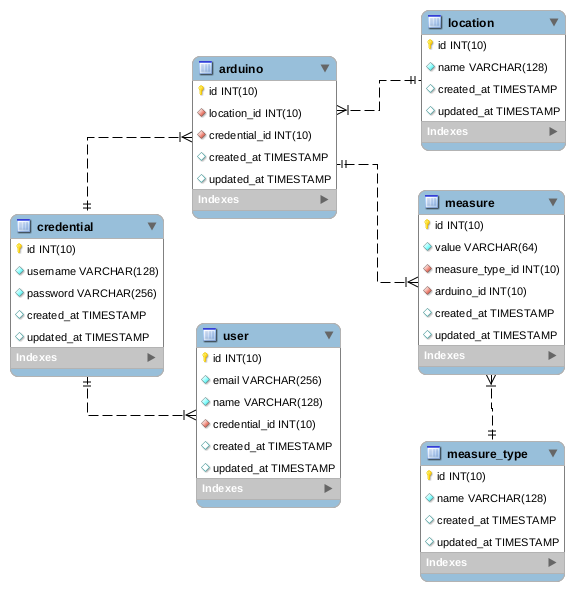
\includegraphics[scale=0.6]{database/scheme.png}
    \hfill
\end{figure}

\section{Atores}

Para representação dos atores foi definida uma tabela chamada credencial, que é utilizada para armazenar os dados de uma entidade que acessa a API.
O arduino é representado por uma localização e por uma credencial, já o usuário possui nome e e-mail, também possuindo uma credencial de acesso.

\section{Entidade de medida}

A representação das medidas no banco de dados é definida pela tabela tipo da medida, que possui qual a medida que é capturada, temperatura, radiação solar, etc.
Também há uma tabela chamada medida, que representa a entidade medida, que possui uma identificação do tipo da medida capturada, do arduino que fez a captura e do valor.

\section{Colunas de marcação de tempo}

Há também as colunas de marcação de tempo em cada uma das tabelas, que são o momento em que o registro foi criado e o momento em que o mesmo foi atualizado, caso o registro nunca tenha sofrido atualização, a coluna de atualização é igual a de criação.
